% use paper, or submit
% use 11 pt (preferred), 12 pt, or 10 pt only

\documentclass[letterpaper, preprint, paper,11pt]{AAS}	% for preprint proceedings
%\documentclass[letterpaper, paper,11pt]{AAS}		% for final proceedings (20-page limit)
%\documentclass[letterpaper, paper,12pt]{AAS}		% for final proceedings (20-page limit)
%\documentclass[letterpaper, paper,10pt]{AAS}		% for final proceedings (20-page limit)
%\documentclass[letterpaper, submit]{AAS}			% to submit to JAS
\usepackage{bm}
\usepackage{amsmath}
\usepackage{subfigure}
%\usepackage[notref,notcite]{showkeys}  % use this to temporarily show labels
\usepackage[colorlinks=true, pdfstartview=FitV, linkcolor=black, citecolor= black, urlcolor= black]{hyperref}
\usepackage{overcite}
\usepackage{footnpag}			      	% make footnote symbols restart on each page
\usepackage{listings}                   % Code Listings
\usepackage[table, x11names]{xcolor}                     % Code Coloring
\usepackage[explicit]{titlesec}         % Paragraph Headers
\usepackage{ulem}                       % Paragraph Headers Underlines

% CREATING PARAGRAPH HEADERS
\titleformat{name=\paragraph,numberless}[runin]
    {\normalfont\normalsize\bfseries}{}{15pt}{\uline{#1}}

% DEFINING CODE COLORS
\definecolor{comments}{rgb}{0.0, 0.5, 0.0}
\definecolor{keywords}{rgb}{0.01, 0.28, 1}

\lstset{
    basicstyle = \small\ttfamily,
    language = Python,
    frame = lines,
    backgroundcolor = \color{lightgray!10},
    commentstyle = \color{comments}\ttfamily\small,
    keywordstyle = \color{keywords}\bf\ttfamily\small,
    framesep=\fboxsep,
}
% \lstset{
%     % language={[LaTeX]TeX},
%     %alsolanguage={PGF/TikZ},
%     frame=single,
%     framesep=\fboxsep,
%     framerule=\fboxrule,
%     % rulecolor=\color{red},
%     xleftmargin=\dimexpr\fboxsep+\fboxrule,
%     xrightmargin=\dimexpr\fboxsep+\fboxrule,
%     breaklines=true,
%     basicstyle=\small\tt,
%     keywordstyle=\color{blue}\sf,
%     % identifierstyle=\color{magenta},
%     % commentstyle=\color{cyan},
%     % backgroundcolor=\color{yellow!10},
%     tabsize=2,
%     columns=flexible,
% }


\PaperNumber{20-686}



\begin{document}

\title{Broad Trajectory Searches Using Monte Carlo Tree Search with the Inclusion of $\Delta$VEGA Trajectories}

\author{Burton A. Yale\thanks{Undergraduate Student, Aerospace Engineering, Cal Poly Pomona, 3801 W Temple Ave, E-mail: bayale@cpp.edu},  
Jehosafat J. Cabrera\thanks{Undergraduate Student, Aerospace Engineering, Cal Poly Pomona, 3801 W Temple Ave, E-mail: jehosafatc@cpp.edu},
\ Rohan D. Patel\thanks{Undergraduate Student, Aerospace Engineering, Cal Poly Pomona, 3801 W Temple Ave, E-mail: rohanpatel@cpp.edu},
\ and Navid Nakhjiri\thanks{Assistant Professor, Aerospace Engineering, Cal Poly Pomona, 3801 W Temple Ave, E-mail: nnakhjiri@cpp.edu}
}


\maketitle{} 		


\begin{abstract}
Multiple flybys of the inner planets and the application of $V_{\infty}$ leveraging are essential trajectory design techniques to reduce the required launch energy for interplanetary missions. These trajectories are often difficult to formulate and require extensive computational resources. However, this problem can be classified as a sequential planning task which can be solved by a Monte Carlo Tree Search (MCTS) method. In this paper, a MCTS algorithm is developed and tested with a focus on reducing required $\Delta$V from the spacecraft. This method balances exploration and exploitation of the search space, and the algorithm’s performance is assessed by tweaking the selection policy parameter. Optimizations of several cases are studied to prove the feasibility of the tree search results. The algorithm will allow for inner-planetary flyby search planning for outer planetary missions.
\end{abstract}

\section{Introduction}
Broad trajectory searches are one fo the first steps in mission planning, allowing for the selection of candidates given a list of constraints and a search space. As is the nature with combinatorial problems, every additional flyby adds another dimension to the search space. Brute force methods lead to expensive but thorough results. By pruning possible choices before the each selection, the overall computation time can be decreased, at the expense of losing possible results. There have been various approaches to this method, from evolutionary/genetic algorithms, to particle swarm optimization, to enumerated searches, all with their own benefits and drawbacks. The method of interest for this algorithm was enumerated searches, a subset of grid searches, as recent work has proven their ability to quickly and accurately find multi-leg interplanetary trajectories\cite{Hennes2015}.

\textbf{M}onte \textbf{C}arlo \textbf{T}ree \textbf{S}earch (MCTS), is a heuristics-based adaptation of the enumerated search, has the ability to both explore and exploit its environment. This allows the algorithm to find the narrow bands where multiple planet combinations are possible and exploit them to complete its goal. As such, larger search spaces can be employed without exponential growth in computation time.

This algorithm will deliver a set of planetary sequences and the dates associated that meet mission criteria, such as destination, launch windows, total fuel budgets, etc. These results can then be passed on to the next phase of the design, optimization 


\section{Background}

Interplanetary mission design is an iterative process. First, a sequence of encounter bodies is selected and is followed by evaluating all possible trajectories for that specified sequence. Due to the increasing complexity of gravity assists and combinatorial solutions, a low-fidelity tool is generally utilized first to find regions of interest. This is then followed by a high-fidelity tool which searches through prospective and highly valued regions.  In literature, this is often referred to as pathfinding and path-solving respectively [3]. Pathfinding is a sequence optimization problem that provides with a diverse set of mission options. Path-solving, on the other hand, embodies a single-leg transfer trajectory optimization problem where two types of transfer models, low-thrust and multi-impulse, are mainly considered [Deep Networks as Approximators of Optimal Transfers Solutions in Multitarget Missions]. Low thrust trajectories can be optimized using direct or indirect methods. Direct methods convert the optimal control problem to a parameter optimization problem through discretization. The optimal solution is then found through nonlinear programming which requires a long computation time. Indirect methods involve solving a two-point boundary value problem using calculus of variations [Practical techniques for low thrust trajectory optimization with homotopic approach]. Artificial Intelligence techniques have been proposed on numerous occasions over the past few decades by a diverse number of scientists as pathfinding algorithms and routines to tackle the multi impulse optimization problem. Some of these techniques include evolutionary algorithms, machine learning, evolutionary neuro-controllers, and tree searches methods [machine learning and evolutionary techniques in interplanetary trajectory design].    

Evolutionary algorithms are optimization routines that make use of heuristics and Darwinian evolution to solve complex optimization problems. Three of the most popular type evolutionary algorithms are genetic algorithms, Differential Evolution (DE), and Particle Swarm Optimization (PSO). DE has been successfully used as an optimization routine to design Halo Orbits and optimal trajectory to Halo Orbits in [Precise Halo orbit Design and Optimal Transfer to Halo Orbits from Earth Using Differential Evolution] and as a interplanetary mission design algorithm [Interplanetary Mission Design Using Differential Evolution].  The Cassini and Galileo missions were considered as case studies to analyze the performance of the algorithm. One each, the DE routine was able to come within appropriate bounds of both trajectories and found minima to the flight constraints applied. PSO was used by Zhuang and Huang in combination with Legendre pseudo-spectral method for solving time-optimal trajectory planning problems. The PSO algorithm was robust enough to handle random initial values but was deemed slow at convergence. Thus, when the change in fitness function of the algorithm is smaller than a predefined value, the searching algorithm is switched the Legendre pseudospectral method for fast convergence [Time-Optimal Trajectory Planning for Under- actuated Spacecraft Using a Hybrid Particle Swarm Optimization Algorithm].  

The application of Machine Learning algorithms to the design of interplanetary trajectory has not been extensively researched as evolutionary or tree search techniques have. The less applicability of these methods to the problems encountered during in trajectory design cause them to not be as effective for use. Machine Learning algorithms require data sets as initializers to the problem. The lack of which throughout the aerospace community as open source information restrict the ability to use these techniques [Machine learning and evolutionary techniques in interplanetary trajectory design]. 

Grid-search, for instance has been previously used as a search algorithm to find possible trajectories to KBOs [4]. Grid search is a type of search algorithm with the ability to map the entire search space so that there are no regions of interest missed. This method has been used to properly parametrize the time of flight between encounter bodies. In this manner, Earth having a period of 365 days will have the same number of possible encounters as Jupiter with a period of approximately 12 years [2]. Thus, the output grid will be that of an angular grid as opposed to a cartesian grid. This type of search algorithm, however, can be expensive in terms of computing power and time. To alleviate both of these constraints, heuristics can be implemented into the program.  

Beam Search (BS), a heuristic tree search algorithm, can be used as a searching criterion to find a sequence of planets from which gravity-assist from [4]. BS uses the method of Breadth-First Search (BFS) to search the tree of possibilities. BS builds each layer of the tree and orders the nodes in accordance to their heuristic cost. However, it only chooses those nodes with a maximum value to build from. Depth-First Search (DPS), alternatively, is used as a searching criterion to traverse down the tree [5]. Opposite to BFS, DPS does not search the tree at every level but rather explores a branch until the termination criteria is met. After which, moving in reverse updates the branch and moves towards the root node to start the process again. Both the BFS and DPS, search and prune the search- space consecutively. Using the Lazy Race Tree Search, the search space is pruned, and nodes ranked through the time of flight [5]. The use of heuristics avoids finding redundant solutions and increases the efficiency of the method used. Izzo et. al. [2] proposed the use of the Monte Carlo Tree Search to find fast solutions to interplanetary trajectories.  

Monte Carlo methods have been suggested extensively for games with a random behavior and minimal observability. The nature of the Monte Carlo methods, however, allow them to be applied to deterministic games with faultless information [A survey of monte Carlo tree search methods]. Starting from the initial state, a large amount of games and actions are simulated until the end of the game. In the majority of cases, actions are chosen at random with no link to the game theory. What this means, is that even if the iterative process is executed for an extended period of time, the move selected and path selected might not the most optimum.  

The search sensitivity criteria of DPS, BS, and BFS are explored in conjunction with that of the MCTS and compared. These searches, however, did not take into account Deep Space Maneuvers (DSMs) and led to trivial solutions when trying to validate the Rosetta Trajectory. The validation and correct recreation of this mission will be the basis of the algorithm taking into account DSMs to fully model Leveraging Orbits. 

\section{Monte Carlo Tree Search Implementation}

This tree is built upon a set of individual nodes, that are all connected to each other through their parent and children, much like a family tree. Each node has an associated state to represent a leg in the tour of a spacecraft, with a planetary body, and the time at which it is encountered. The process of building the tree throughout a run of the algorithm can be characterized by four essential steps: selection, expansion, simulation, and backpropagation. Figure~\ref*{fig:mctsFunc} depicts how the tree changes with respect to each phase of the MCTS loop. 

\textbf{Talk about tree initialization}
%At the start of each iteration, the program will begin at the root of the tree, and select down the tree until a leaf node is reached. From this leaf, the algorithm will expand a set of new child states and choose from the new selection. To generate an expected future reward from this node, the program will conduct a randomly stepped search until termination conditions are met. 
%After a fixed set of iterations of this process has been conducted, the algorithm will gather all leaf nodes, nodes with no children, that meet the user-defined criteria.

\begin{figure}[htb]
	\centering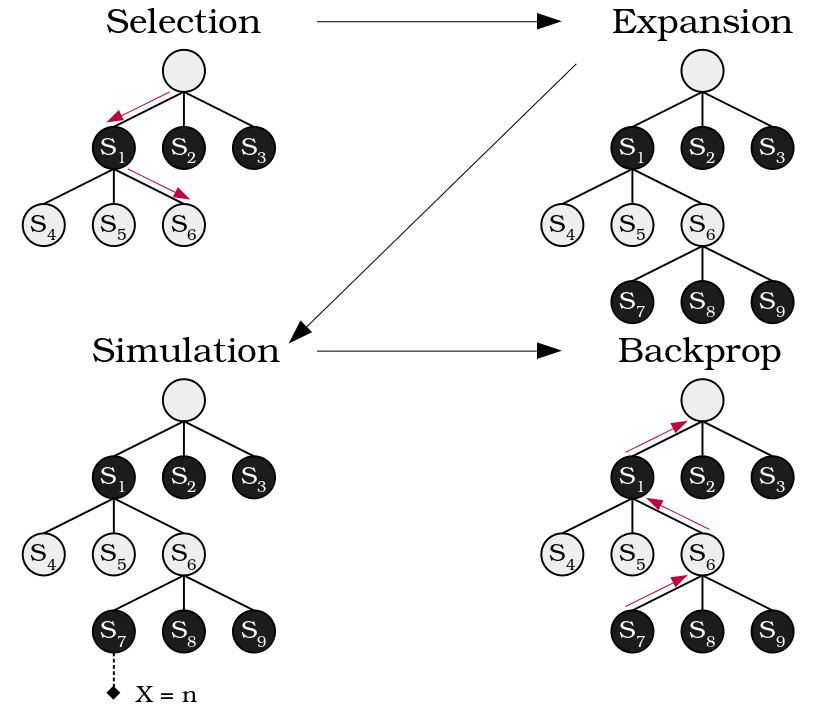
\includegraphics[width=3.5in]{fig/mctsFuncs.png}
	\caption{4 Main Steps for the Creation of a Monte Carlo Tree}
	\label{fig:mctsFunc}
\end{figure}

\subsection{Selection} 
At the start of each iteration, the program begins at the root of the tree $id = 0$, and from its children, select the child with the highest associated UCB1 value. With $X$ being the future reward from exploring the node, $N$ being the number of visits the node has recieved, and $n$ being the number of visits the parent node has recieved. 
\begin{equation*}
    \text{UCB1 Node Value: } X + C_p \sqrt{\frac{\ln{n}}{N}}
\end{equation*}

In the case of $C_p$, the exploration-exploitation parameter, a value of $C_p = \frac{1}{\sqrt{2}}$ was selected due to its performance demonstrated by Hennes \cite{Hennes2015}. 

As the function selects down the tree, it evaluates the all children of each node for is they lead to a terminal condition, such as running out of the fuel budget. If all child nodes are considered terminal, then the associated parent node is also considered terminal, and the function restarts at the top of the tree. This process was implemented in order to prune the tree of any branches that showed results initially, but lead to all terminal states. Once the function has reached a leaf node, it will return the id associated and move onto the next step in building the tree, expansion.

\subsection{Expansion}
Before the creation of the new set of nodes, the function will first look at the state of the current node being expanded from as a base. As planetary motion is a problem involving conic sections, cartesian grid position sampling is not viable, thus angular divisions are required to efficiently sample a planets position. When selecting states for new nodes, the following policy is implemented. 
\begin{equation*}
    E = 
    \left(\begin{array}{c}
        n*(\tau_1 + \tau_0) + t_0 \\ 
        \vdots \\
        m*(\tau_1 + \tau_0) + t_0 \\
    \end{array}\right)
    \text{ for } 
    \left\{\begin{array}{llr} 
        n = 0.1, & m = 1.0 &\text{if } a_1 < 2 \text{ AU} \\ 
        n = 0.05, & m = 0.25 &\text{if } a_1 \geq 2 \text{ AU}
    \end{array}\right.
\end{equation*}

For the ephemeris time array $E$, the time of flight of the Lambert arc is dictated by the period of the planet state of the child node, $\tau_1$, and the period of the planet state of the parent node, $\tau_0$. This array is bounded using the parameters $n$ and $m$, which are defined by the semi-major axis of the child node's planet, $a_1$. The values for $n$ and $m$ were determined based on the performance of the tree, for outer planet destinations, early, faster arrivals were prefered, so their parameters have been reduced to reflect as such. 

With the upper and lower bounds of the array set, an additional parameter, defined by the user, $d$ specifies the length of the array, also defining the resolution of the time steps. For the purpose of this paper, a value of $d = 16$ was found to be sufficient for all calculations as a balance between computation time and detail. 

Once the list of states has been established, a new set of children nodes are created to match all combinations of ephemeris times and planetary id pairs. In order to further prune the tree to reduce unnecessary calculations, Lambert arcs are calculated to each state pair to evauluate their associated $\Delta \text{v}$ cost. Any node that exceeds the mission budget is considered terminal and not used in any further exploration.

In order to calculate mission $\Delta \text{v}$ usage, the simulation uses powered flybys, as characterized by [Wei] \textbf{MORE HERE LATER}
\[ a_\text{in/out} = -\frac{\mu_p}{v^2_{\infty-\text{in/out}}} \]
\[ \delta = \text{cos}^{-1}\left(\frac{ \vec{\textbf{v}}_{\infty-\text{in}} \cdot \vec{\textbf{v}}_{\infty-\text{out}} }{ v_{\infty-\text{in}} \cdot v_{\infty-\text{out}} }\right) \]
\[ f =  \]
\[ \frac{\text{d}f}{\text{d}e_{out}} =  \]
\[ r_p = a_{in}(1 - e_{in}) = a_{out}(1 - e_{out}) \]
\[ \Delta V_{fb} = \left| \sqrt{v^2_{\infty-\text{in}} + \frac{2\mu_p}{r_p}} - \sqrt{v^2_{\infty-\text{out}} + \frac{2\mu_p}{r_p}} \right| \]

From this point, the tree selects the new node with the lowest associated $\Delta V$ cost to continue onto the Simulation step.

\subsection{Simulation}

On the tree's arrival to an unvisited leaf node, the node's future expected reward, $X$, must be calculated. A group of temporary state pairs are expanded from the leaf, as starting point for the random exploration. For each new node, the program will randomly walk through additional state pairs, calculating the $\Delta V$ in the process, until a termination state is reached. When either the budget is expended or the target planet is reached, the associated cost is calculated using the equations below.

\begin{equation}
    \label{eq:simCost1}
    X = \text{max}\left( 0.1 \cdot M,\hspace{0.5em} \frac{\Delta V_{budget} - \Delta V_{used}}{\Delta V_{budget}} \right)
\end{equation}

Upon termination, the reward is balanced between two criteria: $\Delta V$ usage, and number of flybys completed, $M$. In the case were the final desination is not reached, the algorithm will still provide a small benefit to a simulation completing Lambert arcs. After all temporary states have been simulated from, the reward returned from each is averaged and output from the function.

\subsection{Backpropagation}

At the end of the core MCTS loop, Backpropagation communicates the expected reward from a node back up the branch to reflect a more accurate reward of a branch. The $X$ of each node in the branch is adjusted based of a weighted average of its previously observed rewards. 

\begin{equation}
    \label{eq:bp}
    X_{node, new} = \frac{X_{node, old} \cdot N_{node} + X_{new}}{N_{node} + 1}
\end{equation}

Once the cost is propagated up the tree, the loop restarts at another iteration, exploring a new set of state pairs.

\section{$\Delta$VEGA Maneuver Implementation}

A $\Delta$VEGA orbit, also referred to as a leveraging orbit, launches from Earth with the intent to gravity assist off the body for a higher post-flyby heliocentric energy.  Leveraging orbits are classified by their nominal resonance period multiple with respect to Earth's heliocentric orbit, and we will refer to this number as "$k$." For example, a leveraging orbit that has a period roughly 3 times as large as Earth's orbit will have a $k=3$ which is represented as a 3:1 $\Delta$VEGA trajectory. The actual period of these orbits will vary either greater than or less than the nominal time due to flying by the body at a different Earth heliocentric true anomaly. Trajectories with a larger period are referred to as $k$:$1^{+} \Delta$VEGA and those with a shorter are $k$:$1^{-} \Delta$VEGA trajectories. To modify the flyby Earth true anomaly a maneuver at the aphelion (deep space maneuver) is executed.

The deep space maneuver (DSM) and subsequent Earth launch characteristics are calculated before the tree generation in order to reduce the required number of computations within the search. We approximate the $\Delta$V requirements for both maneuvers, and their inclusion reduces the discontinuous trajectory endpoint velocities needed to patch Earth-Earth flyby sequences. Having the required aphelion $\Delta$V can also aid the optimization process initial guess. A lookup table sorted by the nominal resonance multiple ($k$) and encounter true anomalies ($\theta_{E}$) contains the resulting leveraging orbit properties and maneuver magnitudes. Due to being a rough approximation, the circular Earth orbit and coplanar trajectories assumptions are used. Finding the $\Delta$VEGA orbit parameters for a specific encounter true anomaly and $k$ begins by assuming a nominal orbit period launch and its associated $V_\infty$. The state elements are computed at Earth and the resulting aphelion radius and velocity are found. Because the intercept true anomaly is fixed, its location and the time it takes to reach the point are known. Eq.~\eqref{eq:dteqn} is the difference in time from the DSM maneuver location to the Earth gravity assist (EGA) point where $T_E$ is the orbital period of Earth.
%
\begin{equation}
	\label{eq:dteqn}
	dt = kT_E \pm T_E(\theta_E/2\pi)
\end{equation}
%
%
\begin{figure}[htb]
	\centering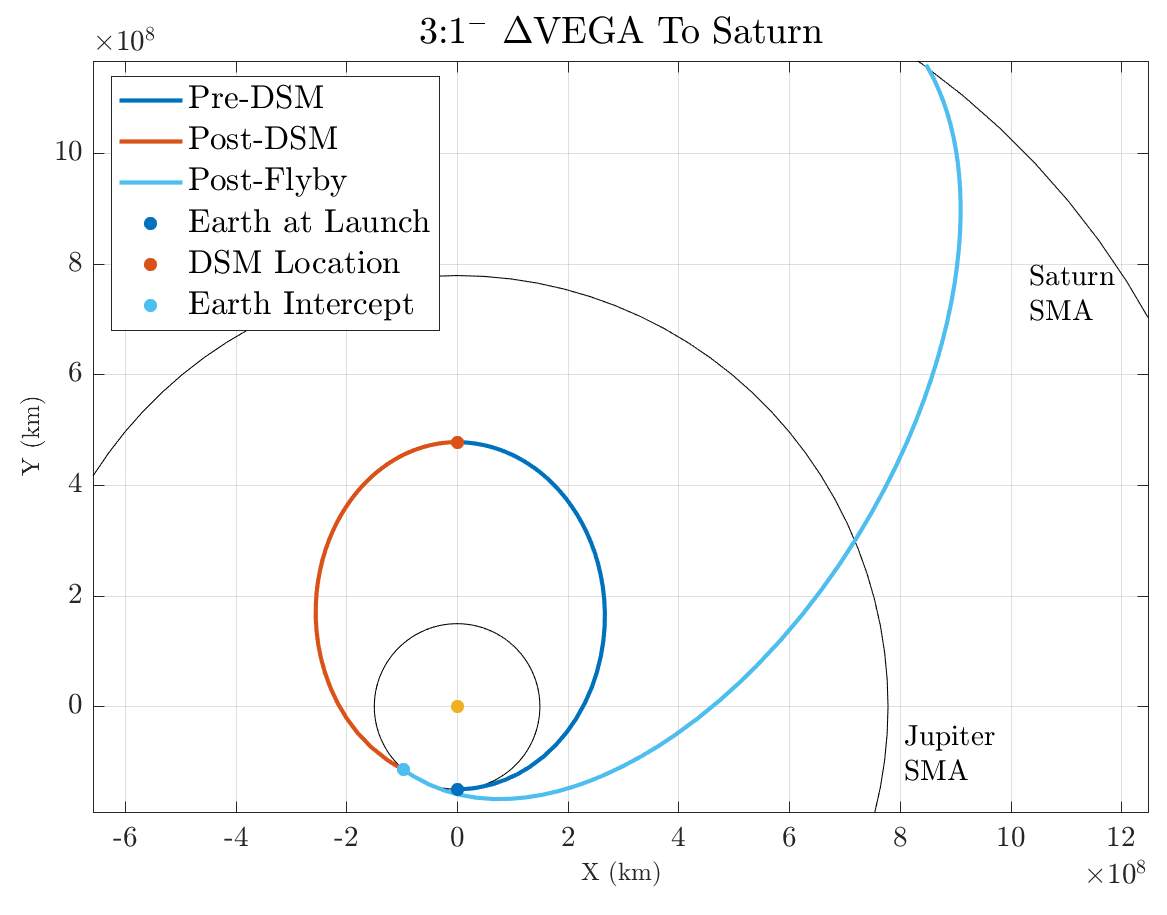
\includegraphics[width=3.5in]{./fig/dsmmatlab}
	\caption{Example of a computed 3:$1^{-} \Delta$VEGA trajectory to Saturn's semi-major axis. The launch $V_\infty$ is 6.97 km/s and the required DSM $\Delta$V is 0.39 km/s. The EGA flyby altitude was constrained to 200 km, which yielded the highest post flyby energy.}
	\label{fig:dsmmatlab}
\end{figure}
%
A Lambert arc is computed between these points and the resulting initially velocity change is used to find the DSM vector. The final velocity vector is assumed to be the heliocentric velocity of the leveraging orbit at the EGA. The relative velocity, $\vec{V_\infty}$ is computed and a planar flyby of Earth can now be calculated from the tree search algorithm. Fig.~\ref{fig:dsmmatlab} illustrates an example leveraging orbit being calculated for $\theta_{E}$ = 40.$7^{\circ}$. An energy maximizing flyby and propagation to the new aphelion is added to the end of the $\Delta$VEGA orbit.
%
From testing, we noticed that as $\mid\theta_E\mid$ increased, a normal component of the DSM $\Delta$V appeared and grew larger. To limit the $\Delta$V to only a tangential component, and in return to reduce the total $\Delta$V required, a minimizer can be employed. This optimization comes at the expense of a higher launch energy and a longer flight time for trajectories with large $\mid\theta_E\mid$. Differing trends from Sims et. al. analysis of $V_\infty$ leveraging\cite{sims1994} were only noticed in high total $\Delta$V cases for each $k$ leveraging orbit family. These solutions were discarded from the lookup table due to delivering lower aphelion radii post-flyby when compared to lower total $\Delta$V leveraging orbits of the same family. The case presented in Fig.~\ref{fig:dsmmatlab} matches that discussed by Sims et. al\cite{Sims1997}.

Now that the $\Delta$VEGA orbit properties are known, the lookup table solution can be extended to the actual solar system model in the tree search. The table values are represented in a relative frame with respect to Earth's state vector at the launch epoch. A subsequent transformation of the departure velocity and pre-EGA incoming $\vec{V_\infty}$ can be done in order to find their specific components corresponding to an Earth epoch in the Ecliptic J2000 frame. From the initial node in the tree, a set of Earth leveraging time-of-flight nodes are created corresponding to their respective $k$ and $\theta_E$ values parameters. The number of these leveraging nodes included in the initial flight time layer of the tree is directly related to the angular spacing of $\theta_E$. As the resolution becomes finer, the estimated $\Delta$V becomes more accurate. This, however, increases of the number of tree nodes created, and so for a rough idea of the trajectory search space, a coarse resolution is preferred. The discontinuous $\Delta$V post-EGA required to patch the incoming leg from the leveraging orbit and outgoing leg to the next planet node will determine if the leveraging node and its performance is effective for the transfer. Using this method, a distinction between the $\Delta$VEGA trajectory families to different outer planets can be observed.

\begin{itemize}
    \item Rohan how dsm's work
    
    \item I talk about how its implemented
\end{itemize}

\section{Performance Evaluation}
\subsection{Europa Clipper Trajectory Recreation}

To validate MCTS's base ability without $\Delta$VEGA orbits, a search was conducted of Europa Clipper's launch window. The goal in mind was to find the EEVEEJ trajectory, as shown by Buffington\cite{Buffington2014}. The nominal trajectory has the spacecraft set to launch on June 03, 2022, and arriving at Jupiter on January 15, 2030 with an additional 3 Earth flybys and 1 Venus flyby.
\begin{table}[htb]
\begin{center}
    \caption{Constrain Input Table for Europa Clipper Trajectory Search}
    \label{table:clipInputs}
    \begin{tabular}{c|c}
        \textbf{Input Name} & \textbf{Input Value}\\
        \hline
        Arrival Planet & Jupiter \\
        Launch Window & March 01, 2022 --- September 01, 2022 \\
        Iterations & 75,000 \\ 
        $\Delta V$ Budget & 10 $km/s$ \\
        Max C3 & 10 $km^2/s^2$ \\
        Detail ($d$) & 24 
    \end{tabular}
\end{center}
\end{table}

Table \ref*{table:clipInputs} provides the search criteria for the broad trajectory search. For general trajectory searches, it was found that an iteration budget of 50,000 was found to be sufficient for most trajectories, but due to the length of the planetary sequence for the nominal trajectory, the iteration limit had to be adjusted. Runs with a $d = 16$ were also conducted, but due to the coarseness in the separation of state pairs, the exact solution was deemed infeasible. As described earlier, this behavior is one of the drawbacks of heuristic searches as not all possible solutions can be found. 

At the completion of the search, the algorithm had conducted 20 million Lambert arcs, and created one million tree nodes. Of the 1.9 billion possible combinations possible for a 6 layer tree, only 275 solutions were deemed feasible for the input criteria. Figure \ref*{fig:clipResults} shows the top 100 trajectories, sorted by their unoptimized mission $\Delta V$. The eighth highest result was the nominal trajectory, with all nodes being within week of the actual planned arrival. The discrepancy is due to the separation of nodes, even at the raised level of detail. Among all top performing trajectories, the initial two flybys of Earth and Venus were held in common sharing similar dates. Of the EEVEEJ solutions found, the most optimal utilized a 3:1 orbital resonance for the final Earth flyby, while the nominal trajectory utilized a 2:1. The 2:1 solutions also exist within the results, but do not appear until later is the data set, utilizing an additional 250 m/s of $\Delta V$. Even with this deviation, the Jupiter arrival occured only one month later than targeted. 


\begin{figure}[htb]
    \begin{subfigure}
        \centering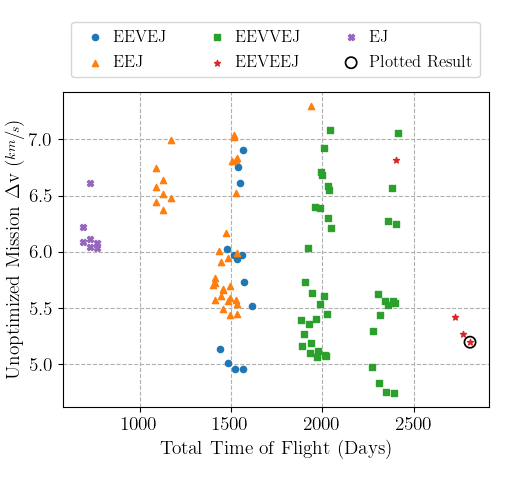
\includegraphics[width=2.75in]{./fig/clipperResults.png}
    \end{subfigure}
    \begin{subfigure}
        \centering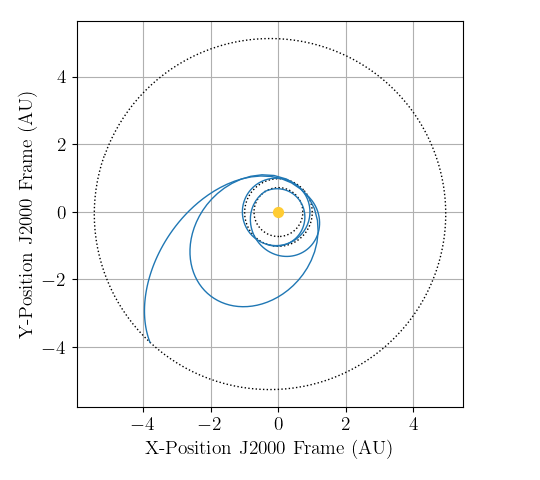
\includegraphics[width=3in]{./fig/clipperMCTS.png}
    \end{subfigure}
    \caption{(Left) Top 100 results from built broad search colored by sequence\hspace{1em} (Right) Circled, unoptimized trajectory from results that matches targeted sequence from Buffington \cite{Buffington2014}}
    \label{fig:clipResults}
\end{figure}

Utilizing the highest performing EEVEEJ transfer, the dates MCTS supplied were optimized using MALTO (Mission Analysis Low Thrust Optimizer) \textbf{REF}. While this tool is primarily designed for low-thrust trajectories, the application is still capable of taking optimizing ballistic and chemical propulsion trajectories. Table \ref*{table:clipMInputs} shows the inputs to MALTO and their associated bounds for the optimizer to search. \textbf{CONTINUE AFTER MALTO SEARCH}

\begin{table}[htb]
    \begin{center}
        \caption{MCTS Results for MALTO Input File ||\textit{I'm not sure if this table is necessary}||}
        \label{table:clipMInputs}
        \begin{tabular}{c|c}
            \textbf{Input Name} & \textbf{Input Value}\\
            \hline
            Launch Date & June 04, 2022 \\
            Earth Flyby \#1 & Jun 02, 2023 \\
            Venus Flyby & November 23, 2023 \\ 
            Earth Flyby \#2 & October 22, 2024 \\
            Earth Flyby \#3 & October 20, 2027 \\
            Jupiter Arrival & February 13, 2030 \\
            Upper \& Lower Bound & $\pm$ 100 days
        \end{tabular}
    \end{center}
\end{table}

\vspace*{3in}
\subsection{Galileo Trajectory Recreation}

\begin{table}[htb]
    \begin{center}
        \caption{Constrain Input Table for Galileo Trajectory Search}
        \label{table:clipInputs}
        \begin{tabular}{c|c}
            \textbf{Input Name} & \textbf{Input Value}\\
            \hline
            Arrival Planet & Jupiter \\
            Launch Window & Jun 01, 1989 --- Dec 31, 1991 \\
            Iterations & 50,000 \\ 
            $\Delta V$ Budget & 10 $km/s$ \\
            Max C3 & 20 $km^2/s^2$ \\
            Detail ($d$) & 16 
        \end{tabular}
    \end{center}
    \end{table}

\begin{figure}[htb]
    \begin{subfigure}
        \centering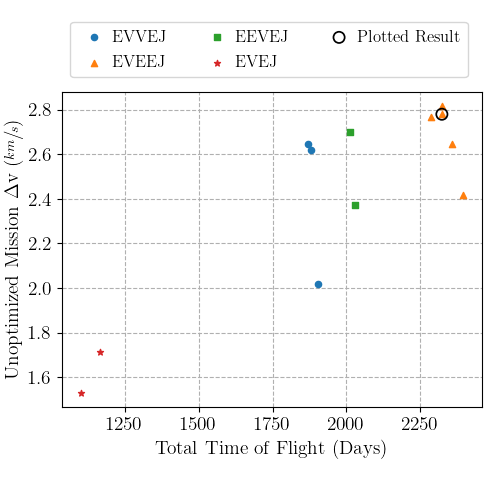
\includegraphics[width=2.75in]{./fig/galileoResults.png}
    \end{subfigure}
    \begin{subfigure}
        \centering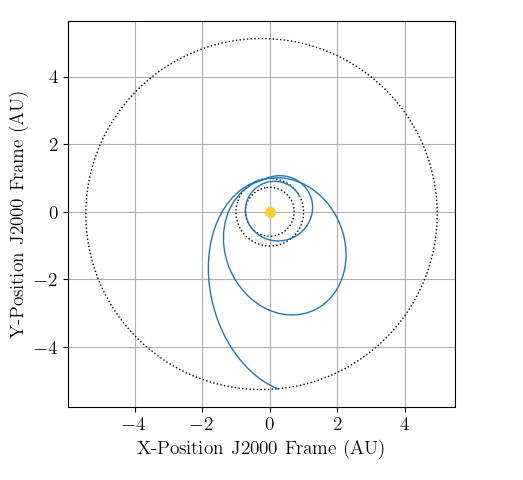
\includegraphics[width=3in]{./fig/galileoMCTS.png}
    \end{subfigure}
    \caption{(Left) Top results from built broad search colored by sequence\hspace{1em} (Right) Circled, unoptimized trajectory from results that matches targeted sequence from D'Amario \cite{DAmario1992}}
    \label{fig:clipResults}
\end{figure}



\subsection{Triton Trajectory Recreation}
Exploratory

\begin{itemize}
    \item Figures
        \item States 
        \item MCTS Trajectory Families
    \item Tables
        \item MCTS Inputs
\end{itemize}

\iffalse
\begin{lstlisting}
def mcts.run():
    for _ in maxIterations:
        if all(launchNodes is terminal):
            break

        # Select Most Valuable Leaf Starting from Root
        id = select() 

        # Expand If Prevously Visited and Pick Most Valuable Child
        if node.children is None and node.visits is not 0:
            id = expand(id)

        # Randomly Explores From Selected Node To Generate Cost
        X = simulate(id) 

        # Propagates Results Up Branch
        backprop(id, X)
\end{lstlisting}
\fi

\appendix
\section{MCTS Run Resutls}
\begin{table}[h!]
    \centering
    \caption{Top 23 results from broad search of Europa Clipper's launch window. Gray row shows nominal solution.}
    \begin{tabular}{l|llllll}
        Result \# & Sequence   & C3 $(\frac{km^2}{s^2})$    & $\Delta V_{unopt} (\frac{km}{s})$   & ToF (Days)            & Arrival $V_\infty (\frac{km}{s})$            \\
        \hline
        0  & EEVVEJ & 3.12  & 4.75 & 2392.28 & 6.62  \\
        1  & EEVVEJ & 3.12  & 5.07 & 2019.14 & 6.30  \\
        2  & EEVVEJ & 3.12  & 5.08 & 2013.15 & 6.36  \\
        3  & EEVEJ  & 3.12  & 4.96 & 1561.77 & 6.54  \\
        4  & EEJ    & 35.83 & 5.44 & 1533.57 & 6.15  \\
        5  & EEJ    & 34.30 & 5.54 & 1533.57 & 6.10  \\
        6  & EEVVEJ & 3.12  & 5.45 & 2025.13 & 6.27  \\
        7  & EEJ    & 28.63 & 5.57 & 1523.57 & 6.17  \\
        \rowcolor{lightgray}8  & EEVEEJ & 3.12  & 5.20 & 2810.10 & 6.58  \\
        9  & EEVVEJ & 3.12  & 4.76 & 2351.48 & 7.02  \\
        10 & EEVVEJ & 3.12  & 5.12 & 1978.34 & 6.71  \\
        11 & EEVVEJ & 3.12  & 5.06 & 1972.34 & 6.76  \\
        12 & EEVEJ  & 3.12  & 4.96 & 1520.96 & 6.94  \\
        13 & EEVEJ  & 3.12  & 5.52 & 1612.78 & 6.41  \\
        14 & EEJ    & 35.83 & 5.44 & 1492.77 & 6.51  \\
        15 & EEJ    & 34.30 & 5.59 & 1492.77 & 6.45  \\
        16 & EEVVEJ & 3.12  & 5.60 & 2007.16 & 6.45  \\
        17 & EEJ    & 28.63 & 5.56 & 1482.76 & 6.53  \\
        18 & EEVVEJ & 3.12  & 5.55 & 2398.27 & 6.57  \\
        19 & EEVVEJ & 3.12  & 5.54 & 1984.33 & 6.66  \\
        20 & EEVVEJ & 3.12  & 5.40 & 1966.35 & 6.84  \\
        21 & EEVVEJ & 3.12  & 5.56 & 2386.29 & 6.68  \\
        22 & EEVEEJ & 3.12  & 5.26 & 2769.29 & 7.01 
    \end{tabular}
\end{table}

\begin{table}[h!]
    \centering
    \caption{All results from broad search of Galileo's launch window. Gray row shows nominal solution.}
    \begin{tabular}{l|lllll}
    Result \# & Sequence   & C3 $(\frac{km^2}{s^2})$    & $\Delta V_{unopt} (\frac{km}{s})$   & ToF (Days)            & Arrival $V_\infty (\frac{km}{s})$            \\
    \hline
    0         & EVEJ  & 19.71 & 1.71 & 1162.28        & 6.64 \\
    1         & EVEJ  & 19.71 & 1.53 & 1099.71        & 7.38 \\
    2         & EVEEJ & 20.75 & 2.42 & 2395.81        & 6.73 \\
    3         & EVVEJ & 19.71 & 2.02 & 1904.48        & 7.27 \\
    4         & EVEEJ & 15.94 & 2.65 & 2360.62        & 6.67 \\
    5         & EEVEJ & 27.93 & 2.37 & 2030.56        & 7.17 \\
    6         & EVEEJ & 28.73 & 2.82 & 2325.42        & 6.72 \\
    \rowcolor{lightgray}7         & EVEEJ & 21.75 & 2.78 & 2325.42        & 6.87 \\
    8         & EEVEJ & 28.97 & 2.70 & 2013.05        & 7.09 \\
    9         & EVVEJ & 15.42 & 2.62 & 1879.77        & 7.24 \\
    10        & EVEEJ & 22.03 & 2.77 & 2289.24        & 7.20 \\
    11        & EVVEJ & 15.42 & 2.65 & 1869.28        & 7.33
    \end{tabular}
\end{table}

\newpage
\bibliographystyle{AAS_publication}   % Number the references.
\bibliography{references}   % Use references.bib to resolve the labels.

\end{document}